\section{Recovering siblings against known groups}
\label{sec:detect}

We evaluate on Leaf-A, Leaf-B and a CIFAR-Aug subset of $500$ sources, $50$ from each of the ten classes ($8{,}000$ images per strength), whose groups are known. Every method is turned into links the same way (hubness correction, label-calibrated null, $p<\alpha$), so the comparison isolates the similarity. Baselines are byte hashes, the perceptual hash~\citep{zauner2010phash} with and without dihedral search, and the frozen ImageNet embedding (with its dihedral orbit average). We also test a self-supervised \emph{invariant embedding}: a linear projection of the frozen embedding fitted on the release itself, which keeps directions that separate photographs and discards directions that a fixed, generic family of edits moves (a Fisher criterion with synthetic copies as classes; Appendix~\ref{app:invariant}). It uses no labels or groups, and the edit family is the same for every dataset.

\begin{table}[t]
\centering\small
\setlength{\tabcolsep}{4pt}
\caption{\textbf{Recovering siblings against known groups.} AP: average precision over all image pairs. Hit: share of images linked to at least one true sibling at $\alpha=10^{-3}$. Best per column in bold. File-name groups in Leaf-A/B miss repeat shots of the same leaf (Section~\ref{sec:audit}), so precision there is a lower bound.}
\label{tab:detect}
\begin{tabular}{@{}lcccccccccc@{}}
\toprule
 & \multicolumn{2}{c}{Leaf-A} & \multicolumn{2}{c}{Leaf-B} & \multicolumn{2}{c}{C-Aug weak} & \multicolumn{2}{c}{C-Aug medium} & \multicolumn{2}{c}{C-Aug strong} \\
\cmidrule(lr){2-3}\cmidrule(lr){4-5}\cmidrule(lr){6-7}\cmidrule(lr){8-9}\cmidrule(lr){10-11}
method & AP & hit & AP & hit & AP & hit & AP & hit & AP & hit \\
\midrule
pHash & 0.38 & 56 & 0.55 & 74 & 0.50 & \textbf{100} & 0.03 & 3 & 0.01 & 1 \\
pHash, dihedral search & 0.44 & 63 & 0.64 & 79 & \textbf{1.00} & \textbf{100} & 0.04 & 6 & 0.01 & 1 \\
ImageNet embedding & 0.03 & 8 & 0.20 & 11 & \textbf{1.00} & \textbf{100} & 0.62 & 43 & 0.07 & 5 \\
invariant embedding & 0.10 & 28 & 0.49 & 74 & \textbf{1.00} & \textbf{100} & 0.66 & \textbf{74} & 0.07 & \textbf{9} \\
structure view & 0.51 & 55 & 0.72 & 54 & \textbf{1.00} & 39 & 0.48 & 23 & \textbf{0.12} & 3 \\
AugLeak (structure + hash) & \textbf{0.57} & \textbf{81} & \textbf{0.76} & \textbf{83} & \textbf{1.00} & \textbf{100} & 0.42 & 26 & 0.09 & 4 \\
AugLeak (+ invariant) & 0.52 & 80 & -- & -- & \textbf{1.00} & \textbf{100} & \textbf{0.71} & 70 & 0.11 & \textbf{9} \\
\bottomrule
\end{tabular}
\end{table}


\paragraph{AugLeak is best on both real releases; ImageNet embeddings are worst.}
Table~\ref{tab:detect} and Figure~\ref{fig:detect} show that AugLeak's two pixel views together reach the highest average precision on Leaf-A (\numDetLeafApixAP{}) and Leaf-B (\numDetLeafBpixAP{}), ahead of either view alone and of perceptual hashing. The ImageNet embedding, a common tool for de-duplication, is the weakest method on both (AP \numDetLeafAsemAP{} and \numDetLeafBsemAP{}). Its failure is systematic, not noisy (Figure~\ref{fig:detect}e): filtered copies embed close to copies of \emph{other} photographs made with the same filter. The invariant projection repairs most of this from the release alone, but not for grayscale, rotation and morphological filters. Top-hat and black-hat copies defeat every method, and rotated copies are found less than half the time.

\paragraph{The right view depends on the edits.}
On CIFAR-Aug, where copies are random crops of $32\times32$ images, the pixel views are weak and the invariant view is strong. Adding it gives the best AP at medium strength (\numDetCmediumallAP{}). With weak edits every method that searches flips is near perfect. With strong edits (crops, rotations and filters at once, on tiny images) no method recovers most pairs.

\paragraph{Calibration.}
On CIFAR-Aug, AugLeak's pixel views are conservative (Figure~\ref{fig:detect}d): at every strength and $\alpha$, the share of images linked to a same-class non-sibling stays below $\alpha$. Adding the invariant view raises it to $5\times\alpha$ at $\alpha=10^{-4}$ (medium edits), because unrelated photographs of one class are close in an ImageNet embedding, which the label null does not see; we keep that view optional. The null also needs enough classes: on a three-class subset the pixel views' rate rose to $1.5$--$60\times\alpha$ (Appendix~\ref{app:hyper}). On the three-class leaf releases the rate is far higher, but most of these ``false'' links join different source photographs of the \emph{same physical leaf}, taken moments apart (Section~\ref{sec:audit}).

\paragraph{Pairs are not groups.}
As Proposition~\ref{prop:frag} predicts, splitting by detected components leaves most test images nominally exposed on every release, because groups fragment (Appendix Table~\ref{tab:resid}).

\begin{figure}[t]
  \centering
  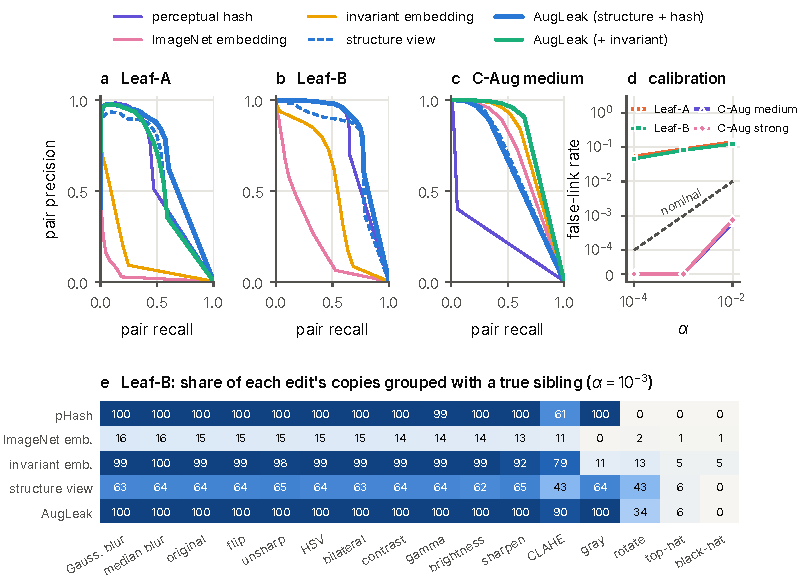
\includegraphics[width=\linewidth]{figs/fig_detect.pdf}
  \caption{\textbf{Sibling recovery with ground truth.} (a--c) Pairwise precision--recall over all image pairs (average precision in Table~\ref{tab:detect}). (d) Calibration of AugLeak: share of images linked to a same-class non-sibling, against the nominal $\alpha$; on the leaf releases most such links join repeat shots of the same leaf. (e) Leaf-B: share of each edit's copies that end up in a detected group with a true sibling, at $\alpha=10^{-3}$.}
  \label{fig:detect}
\end{figure}
